%!TEX program = xelatex
% 完整编译: xelatex -> bibtex -> xelatex -> xelatex
\documentclass[lang=cn,11pt,a4paper,cite=numbers]{elegantpaper}

% 本文档命令
\usepackage{float}


\begin{document}

\tableofcontents
\newpage

\section{文献综述}

\subsection{Abstract}

Currently, the number of people suffering from cardiovascular diseases(CVD) in China is about 290 million, and the number is still increasing year by year. In addition to the risk of death, the high morbidity and disability rates of cardiovascular diseases impose a heavy economic and psychological burden on society, families and individuals. Among them, coronary artery disease (CAD) is the most common cardiovascular disease. Accurate coronary artery segmentation is very important for the diagnosis and treatment of coronary artery disease. However, coronary artery structure is thin and small, and may be accompanied by lesions caused by stenosis, therefore it is difficult to get efficient and accurate segmentation. To address this problem, researchers have tried various methods to reduce the segmentation difficulty, while improving the accuracy and efficiency. Traditional segmentation algorithms are mostly designed based on the correlation between pixels or the structure features of vessels. In recent years, with the development of machine learning, training neural network for coronary artery segmentation has become a research hotspot. In this survey, we review and classify the methods of coronary artery segmentation. For each method, we introduce its techniques and the segmentation results. We conclude the survey by discussing the future directions.

\textbf{Keywords:} coronary artery segmentation, medical image, neural network, traditional methods

\subsection{Introduction}

Cardiovascular disease is one of the most serious health problems in China and even in the world, and the majority of all cardiovascular diseases can be attributed to coronary artery problems. Therefore, the task of coronary artery segmentation is very important.

The coronary artery is the blood vessel that sits at the top of the heart and grows around it, which is shaped like a crown. It is the artery that supplies blood to the heart. A well-flowing coronary artery ensures that the heart has enough nutrients to keep itself moving. Coronary artery disease is mostly caused by the stenosis of the left or right artery, and the purpose of coronary artery segmentation is to more clearly extract the shape, thickness and other characteristics of the coronary artery for further analysis, diagnosis and treatment.  At present, advanced cardiac imaging technology has become an important tool to help doctors treat heart disease. However, the regular review of images takes considerable time and requires a high level of expertise from doctors. Coronary artery segmentation, which can greatly simplify the review process, has received greater attention.
	
However, the structure of coronary artery is extremely complex and hard to segment. The diameter of coronary artery is only 2mm-5mm, and even 1mm in stenosis area. It also has many thin and tiny vessel branches. To achieve coronary artery segmentation, traditional methods include regional-growing approaches, level-set methods, centerline-based methods, etc. In recent years, machine learning method has shown its advantages in various fields, so many researchers also begin to train neural network to segment the coronary artery.
	
In this survey, we focus on various methods of coronary artery segmentation. We divide them into traditional methods and machine learning methods. For each method, we introduce its techniques and the segmentation result. The rest of the paper is organized as follows. In Section 2, we review traditional coronary artery segmentation methods, and In Section 3, we focus on deep learning methods. Finally, in Section 4, we put forward the research challenges and future directions.


\subsection{Traditional methods of coronary artery segmentation}

Traditional coronary artery segmentation methods include regional-growing method, level-set method, Frangi’s vesselness filter, center-line based method, etc. These segmentation algorithms are mostly designed based on the correlation between pixels or the structure features of vessels, using mathematical techniques to extract vessels features. 

\subsubsection{Regional-growing approaches}

Reginal-growing approaches are suitable for the extraction of coronary vessels, which are dendritical structures. The basic idea of region growing is to search the intravascular pixels from the selected seed points, then add the suitable pixels iteratively to the blood vessel regions according to a predefined growth criterion. The intensity similarity is a basic growing criterion for the image segmentation, which considers the pixels with similar intensities to be from the same object. In recent years, many researchers try combining region growing technique with other algorithms to get satisfying results.

% todo 区域生长的算法的过程描述
\begin{figure}[H]
    \centering
    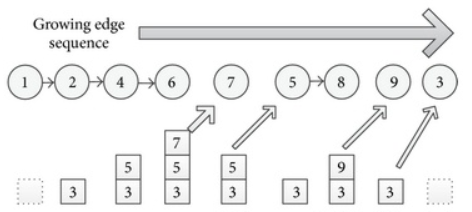
\includegraphics[scale=1]{./image/文献综述/区域生长.png}
    \caption{Process description of the algorithm of region growth}
    \label{fig:RegionGrowth}
\end{figure}

In \emph{A coronary artery segmentation method based on multiscale analysis and region growing - ScienceDirect}\cite{1}, a method of region growing and multi-scale analysis is proposed to extract coronary artery vessels. The method takes advantages of multiscale Hessian analysis strength, defining a robust new region growing criterion tailored to the coronary artery segmentation problem. This method successfully avoid the problem of vascular loss when the intensity of blood vessels is low caused by plaques, but will result in over- or under-segmentation. A completely automated algorithm to segment coronary artery and extract centerline has been proposed in \emph{Region based coronary artery segmentation using modified Frangi's vesselness measure}\cite{2}. It gets seed points automatically, and segment the left and right coronary arteries respectively using region growing method. In \emph{A coronary artery segmentation method based on region growing with variable sector search area}\cite{3}, a region growing method based on variable sector region searching is proposed. The method successfully segment complicated coronary structures. Further validation studies of stenoses detection and catheter removal may be required of this work.

Regional-growing methods segment the connected regions with the same characteristics, and provide good boundary information and segmentation results.  However, native region growing technique also has some disadvantages: (1) it needs manual interaction to obtain seed points; (2) it is sensitive to noise; (3) the problem of over-segmentation will occur as a result of partial volume effect.

\subsubsection{Level-set methods}

Level Set Method (LSM) is a numerical technique for interface tracing and shape modeling. It is used for numerical calculation of evolving curves and surfaces, tracking the topological structure changes of objects. It has a good performance in the task of coronary artery segmentation.

% todo 水平集算法对曲面建模
\begin{figure}[H]
    \centering
    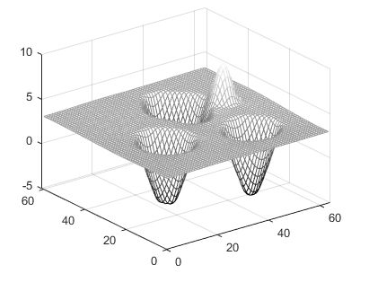
\includegraphics[scale=1]{./image/文献综述/水平集.png}
    \caption{Level set algorithm for surface modeling}
    \label{fig:LevelSet}
\end{figure}

In \emph{Coronary Artery CT Image Segmentation Based on Level Set Method}\cite{4}, a method of coronary artery CT image segmentation based on LSM is proposed. The results show that compared with manual method, the reconstruction time of level set method is reduced by about 10 times, and the fractional flow reserve (FFR) value is satisfying. However, this method required manual mark of the range of the target coronary artery area. In \emph{Segmentation of Coronary Artery Using Region Based Level Set with Edge Preservation}\cite{5}, a level set method for segmentation of coronary artery is presented. In this method, local intensity information is introduced into the level set formulation where the bias field is estimated by a linear combination of a given set of orthogonal basis functions. This method reduces miss- and over-segmentation caused by noise.

The advantage of the level set method is that evolving curves and surfaces is numerically calculated on a Cartesian grid without having to parameterize them. Another advantage of the level set method is that it is easy to track changes in the object's topology.

\subsubsection{Frangi's vesselness filter}

Frangi's vesselness filter is an edge detection enhanced filtering algorithm based on Hessian matrix. It is sensitive to round tubular structures. When the scale of vessels is set, it segments those vessels which fit the bill. Therefore, it is well suited for coronary artery segmentation. \emph{Region based coronary artery segmentation using modified Frangi's vesselness measure}\cite{6} presents a fully automated method for coronary artery extraction using modified Frangi's vesselness measure and region based segmentation. In this method, grayness and gradient based measures are used while computing Frangi's vesselness measure to improve the extraction of coronary arteries.

Frangi's filter is good at segmenting blood vessels, but the scale needs to be set artificially, and it also segments the blood vessels in the lungs, requiring additional post-processing. 

\subsubsection{Other related methods}

Besides those methods stated above, there are also many other traditional methods for coronary artery segmentation. In \emph{Automatic centerline extraction of coronary arteries in coronary computed tomographic angiography}\cite{7}, a fully automatic coronary artery extraction method for CCTA images is presented, which mainly relies on an improved Frangi's vesselness filter. This method is centerline-based, and extract coronary arteries in CCTA images with excellent performances in extraction ability and accuracy. \emph{Deformable tree models for 2D and 3D branching structures extraction}\cite{8} proposes a deformable tree model for coronary artery segmentation, which is validated on 2D MR angiography images and 3D CT data. \emph{Tracking Elongated Structures using Statistical Snakes}\cite{9} introduces a statistic snake that learns and tracks image features by means of static learning techniques. In this approach, a sound statistical model is introduced to define a likelihood estimate of the grey-level local image profiles together with their local orientation. Each of these methods has its own advantages and disadvantages. In fact, there are still many problems need to deal with in the task of coronary artery segmentation.

\subsection{Deep-learning based methods of coronary artery segmentation}

Deep learning has had a tremendous impact on various fields of computer vision, particularly approaches for medical image segmentation. In the field of coronary artery segmentation, different types of neural networks are applied as tools for deep learning. Apart from that, tree structures and graphical connectivity have been introduced as prior knowledge in coronary artery centerline extraction and other approaches. In recent years, some more strategies have been taken on the stage, namely weakly-supervised segmentation and knowledge transfer.

\subsubsection{Variants of networks}

\paragraph{Convolutional Neural Network(CNN)}

Convolutional neural network is a special kind of multilevel perceptron architecture, where an input image passes through a sequence of classification tests that can extract and recognize its consistent intensity patterns and finally make a prediction about the image according to these patterns. The way how CNN works is to extract and recognize patterns in images through the layers and functions to make judgments about the special features in it. The process is based on learning from a large number of image datasets whose special features are already highlighted. 

% todo CNN网络结构
\begin{figure}[H]
    \centering
    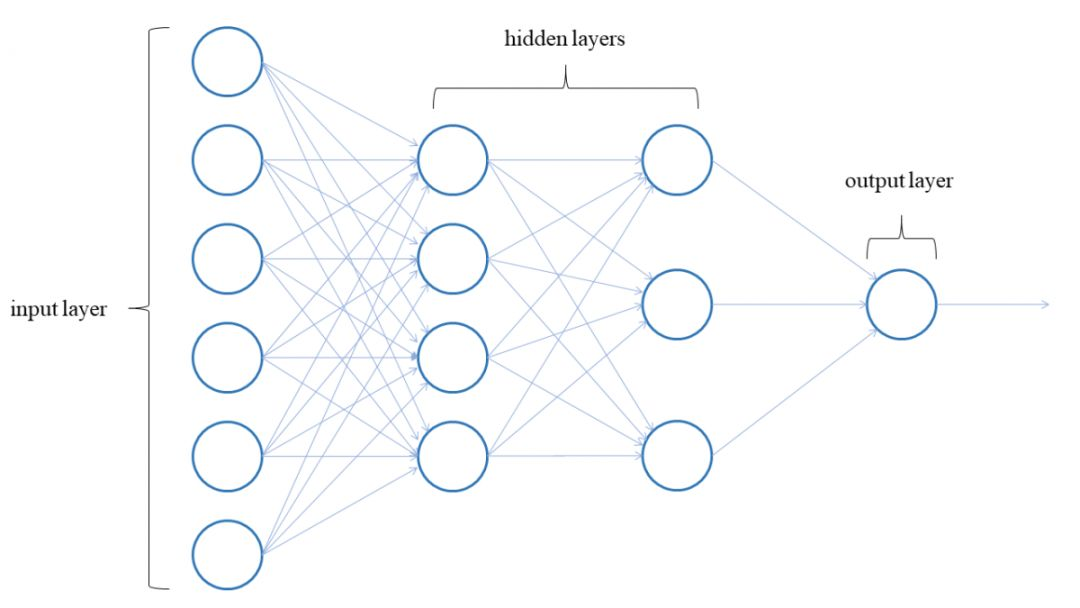
\includegraphics[scale=0.5]{./image/文献综述/CNN.jpg}
    \caption{CNN network structure}
    \label{fig:CNN}
\end{figure}

In \emph{Multi-Resolution 3D Convolutional Neural Networks for Automatic Coronary Centerline Extraction in Cardiac CT Angiography Scans}\cite{10}, a 3D CNN is trained to predict the most likely direction and radius of an artery at any given point in a cardiac CT angiography(CCTA) image based on a local image patch. Starting from a single seed point placed manually or automatically anywhere in a coronary artery, a tracker follows the vessel centerline in two directions using the predictions of the CNN. Tracking is terminated when no direction can be identified with high certainty. The CNN is trained using manually annotated centerlines in training images. The proposed method is able to accurately and efficiently determine the direction and radius of coronary arteries based on information derived directly from the image data. 

With shared convolutional kernel, CNNs can easily deal with high-dimensional data. However, instead of images, the output of CNNs is usually numbers or vectors, which loses two-dimensional features. Other disadvantages of CNN are mainly high storage and low computational efficiency.

\paragraph{Fully Convolutional Network(FCN) and U-Net}

An FCN has a structure slightly different from a CNN, with a fully-connected layer changed into a convolutional layer. Medical image formats are diverse, and FCN can input images of any size. The newly-added skip connection structure ensures both robustness and accuracy of the network. 

% todo FCN的网络结构
\begin{figure}[H]
    \centering
    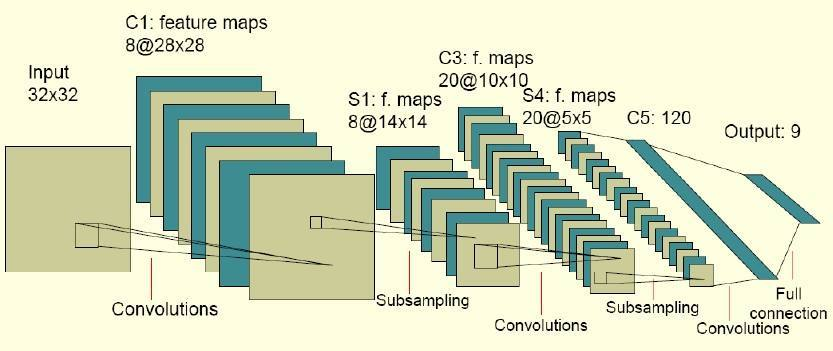
\includegraphics[scale=0.6]{./image/文献综述/FCN.jpg}
    \caption{FCN network structure}
    \label{fig:FCN}
\end{figure}

A relatively new architecture on the basis of FCN is called U-Net convolutional network, dedicated to biomedical image analysis, which performs better in medical images. U-Net combines CNNs and data enhancement technology to increase the amount of medical data. Divided into encoder part and decoder part, the U-Net’s U-shaped structure and layer jump connection make it possible to better extract high-level semantic information and preserve low-level structural features. 

On the basis of U-Net, Lien Kamp et al. introduced the 3D U-Net in 2016 in \emph{3D U-Net: Learning Dense Volumetric Segmentation from Sparse Annotation}\cite{11}. After improvements, the 3D U-Net can input three-dimensional images, which has good versatility. Zhou et al. introduced the U-Net++ in 2018 in \emph{UNet++: A Nested U-Net Architecture for Medical Image Segmentation}\cite{12}, which reduces the semantic gap between the feature maps of the encoder and decoder sub-networks. Finally, in 2020 in \emph{Automated Design of Deep Learning Methods for Biomedical Image Segmentation}\cite{13}, Fabian Isensee et al. Proposed nnU-net, which automatically adapts to distinctive datasets and, in terms of huge-amount tasks, surpasses networks specialized for some certain segmentation missions.

% todo Unet的网络结构
\begin{figure}[H]
    \centering
    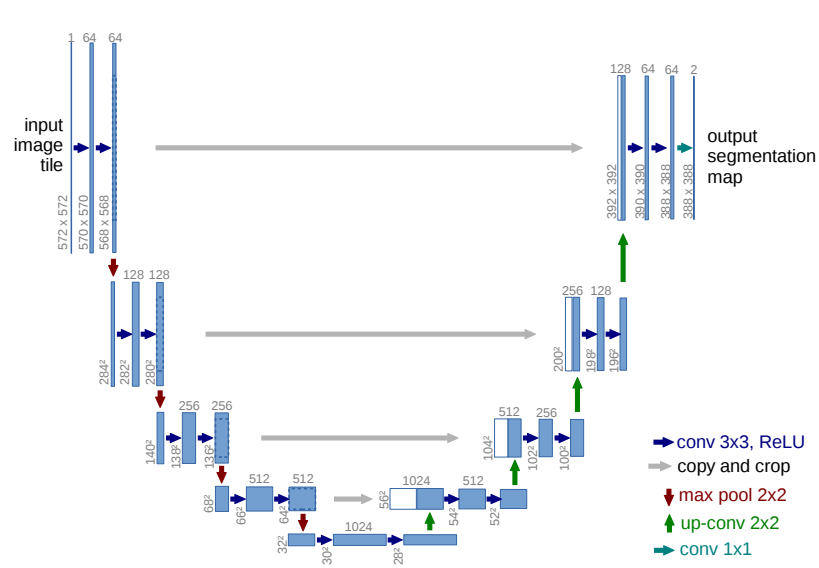
\includegraphics[scale=0.6]{./image/文献综述/UNET.png}
    \caption{UNET network structure}
    \label{fig:UNET}
\end{figure}

Extracting coronary artery centerline from a segmentation mask faces multiple notable challenges, namely multiple branches and significant branch diameter changes. To address such problems, in \emph{DeepCenterline: A Multi-task Fully Convolutional Network for Centerline Extraction}\cite{14}, a two-head multi-task FCN is proposed which simultaneously generates a locally normalized distance map and a list of branch endpoints. The multi-task FCN accomplishes two tasks: computing a normalized centerline distance map and detecting branch endpoints. Skip-connections are added among features of same scale to facilitate good use of information.

In \emph{Coronary Artery Segmentation in Cardiac CT Angiography Using 3D Multi-Channel U-net}\cite{15}, 3D U-Net is applied in extraction of coronary artery area from Computed Tomographic Angiography (CTA). To overcome the difficulties caused by attenuation ambiguity, a 3D multi-channel U-Net architecture is proposed for fully automatic 3D coronary artery reconstruction from CTA. Other than using the original CTA image, the main idea of the approach is to incorporate the vesselness map into the input of the U-Net, which serves as the reinforcing information to highlight the tubular structure of coronary arteries.

\paragraph{Graph Convolutional Network(GCN)}

GCNs are a recent development in deep learning-based medical image analysis, applied mostly in Non Euclidean Structure where CNNs may perform unsatisfactory results. They have high potential for graph-based applications in airway extraction in chest CT and cortical segmentation. The GCN consists of layers that aggregate information from neighboring nodes. By concatenating several such layers, information from a growing neighborhood of nodes in the graph is combined.

% todo 图形卷积网络的结构
\begin{figure}[H]
    \centering
    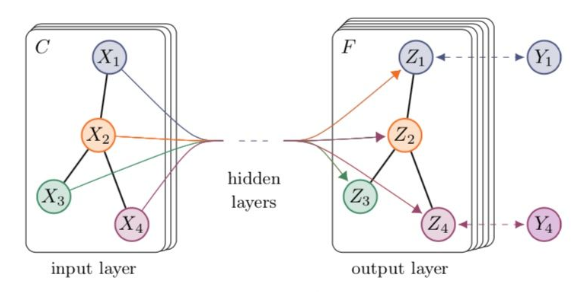
\includegraphics[scale=0.8]{./image/文献综述/图形卷积网络.png}
    \caption{GCN network structure}
    \label{fig:GCN}
\end{figure}

In \emph{Graph Convolutional Networks for Coronary Artery Segmentation in Cardiac CT Angiography}\cite{16}, GCNs are used to obtain a coronary artery surface mesh based on a CCTA image and an automatically extracted coronary artery centerline, to predict the spatial location of vertices in a tubular surface mesh that segments the coronary artery lumen. Predictions for individual vertex locations are based on local image features as well as on features of neighboring vertices in the mesh graph.

\paragraph{Graphical adversarial network(GAN)}

For image segmentation tasks, networks usually predict the category of each pixel at the pixel-wise. The segmentation results may lack continuity and obviously differ from the ground-truth, because deep networks usually ignore the correlation between pixels. In \emph{UENet: A Novel Generative Adversarial Network for Angiography Image Segmentation}\cite{17}, Xiaotong Shi et al. explore to use generative adversarial mechanism to deal with the above problems. GANs can be treated as a competitive procedure between the generator and the discriminator. 

Two problems will be handled with conditional generative adversarial networks (cGANs): blood vessel discontinuity and intra-class inconsistency. To extract better feature of fine coronary arteries in angiography imaging, cGAN was modified to achieve the artery segmentation.

\paragraph{PSPNet}

Using an image block around the pixel as the input of the CNN network for training and prediction is the characteristic of traditional CNN-based segmentation methods. This method has several disadvantages, namely requiring a lot of storage space, long segmentation time and others. FCN overcomes the above shortcomings by recovering the category to which each pixel belongs from the abstract features, but it does not fully consider the relationship between pixels. Ignore the spatial regularization step used in the usual pixel classification-based segmentation method, which makes the network lack of spatial consistency.

In \emph{Semantic Image Segmentation with Deep Convolutional Nets and Fully Connected CRFs}\cite{18}, Zhao et al. proposed Pyramid Scene Parsing Network (PSPNet). After feature extraction was performed on the input data, they input the feature map into the pyramid pooling module, and finally cascaded to get the feature surface, and then learned and adjusted the parameters by calculating the loss and back propagation algorithm. Compared with Global Pooling, this structure is better for obtaining multi-size global information.

In \emph{Coronary angiography image segmentation based on PSPNet}\cite{19}, Zhu et al. proposed segmentation of coronary angiography images based on PSPNet network, which was compared with FCN, and analyzed and discussed the experimental results using three evaluation indicators of precision, recall and Fl-score. Aiming at the complex and changeable structure of coronary angiography images and over-fitting or parameter structure destruction, they implemented the parallel multi-scale convolutional neural network model using PSPNet, using small sample transfer learning that limits parameter learning method.

\subsubsection{Deep-learning prior knowledge}

When deep-learning is applied in multi-classification tasks, the models are often complex and time-consuming. To address such problem, methods combining prior knowledge and deep-learning have been put forward. Prior knowledge is the object structures manually set and inserted in the network before training, so that deep-learning receives better results in less time. Tree and graphical structures are mainly used in coronary artery segmentation.

\paragraph{Tree structures}

Inspired by recent ideas to use tree-structured long short-term memory (LSTM) to model the underlying tree structures for NLP tasks, in \emph{Learning Tree-Structured Representation for 3D Coronary Artery Segmentation}\cite{20}, Bin et al. proposed a novel tree-structured convolutional gated recurrent unit(ConvGRU) model to learn the anatomical structure of the coronary artery. Their tree-structured model considers the local spatial correlations in the input data as the convolutions are used for input-to-state as well as state-to-state transitions, thus more suitable for image analysis. To conduct voxel-wise segmentation, a tree-structured segmentation framework is presented. It consists of a fully convolutional network for multi-scale discriminative feature extraction and the final prediction, and a tree-structured ConvGRU layer for anatomical structure modeling.

% todo 树结构模型
\begin{figure}[H]
    \centering
    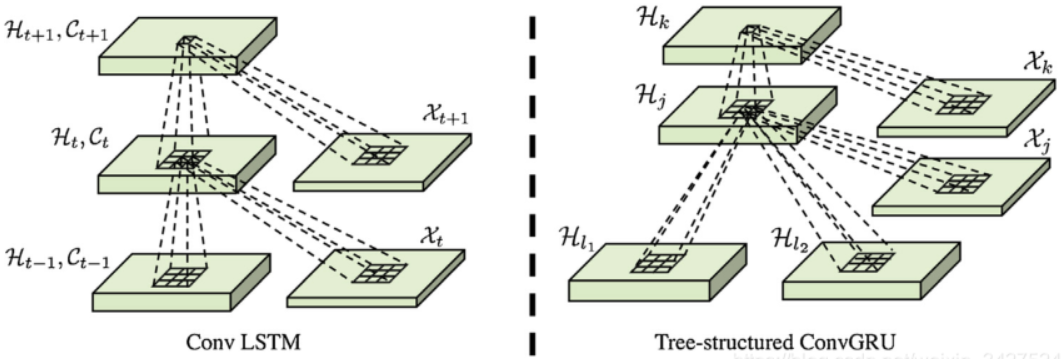
\includegraphics[scale=0.5]{./image/文献综述/树结构.png}
    \caption{Tree structure model}
    \label{fig:Tree}
\end{figure}

\paragraph{Graphical structures}

Existing methods using CNNs have mostly relied on local appearances learned on the regular image grid, without consideration of the graphical structure of vessel shape. Effective use of the strong relationship that exists between vessel neighborhoods can help improve the vessel segmentation accuracy. In \emph{Deep Vessel Segmentation By Learning Graphical Connectivity}\cite{21}, Shin et al. incorporated a graph neural network into a unified CNN architecture to jointly exploit both local appearances and global vessel structures. They extensively performed comparative evaluations on four retinal image datasets and a coronary artery X-ray angiography dataset, showing that the proposed method outperforms or is on par with current state-of-the-art methods in terms of the average precision and the area under the receiver operating characteristic curve.

\subsubsection{Deep-learning strategies}

As the structure of coronary artery is extremely complex and hard to segment, some strategies have been proposed to meet the standard of less training datasets, better segmentation results.

\paragraph{Weakly-supervised segmentation}

The segmentation of coronary arteries in X-ray angiograms by convolutional neural networks is promising yet limited by the requirement of precisely annotating all pixels in a large number of training images, which is extremely labor-intensive especially for complex coronary trees. To alleviate the burden on the annotator, in \emph{Weakly Supervised Vessel Segmentation in X-ray Angiograms by Self-Paced Learning from Noisy Labels with Suggestive Annotation}\cite{22}, Zhang et al. proposed a novel weakly supervised training framework that learns from noisy pseudo labels generated from automatic vessel enhancement, rather than accurate labels obtained by fully manual annotation. They proposed an annotation-refining self-paced learning framework (AR-SPL) to correct the potential errors using suggestive annotation. An elaborate model-vesselness uncertainty estimation was also proposed to enable the minimal annotation cost for suggestive annotation, based on not only the CNNs in training but also the geometric features of coronary arteries derived directly from raw data.

\paragraph{Knowledge Transfer}

As is mentioned in the former section, classic unsupervised methods fail to produce satisfactory results and modern supervised learning requires manual annotation which is often time-consuming and can sometimes be infeasible. In \emph{Annotation-Free Cardiac Vessel Segmentation via Knowledge Transfer from Retinal Images}\cite{23}, Yu et al. proposed a knowledge transfer based shape-consistent generative adversarial network (SC-GAN), which is an annotation-free approach that uses the knowledge from publicly available annotated fundus dataset to segment coronary arteries, known as knowledge transfer. The proposed network is trained in an end-to-end fashion, generating and segmenting synthetic images that maintain the background of coronary angiography and preserve the vascular structures of retinal vessels and coronary arteries.

\subsection{Future directions and developments}

In the following sections, we discuss in detail the potential future research directions for semantic segmentation of coronary artery.

\subsubsection{Combined traditional and deep-learning direction}

We conclude that compared with deep-learning methods, traditional methods are more dependent on prior knowledge and make full use of coronary and vessel structures. As a comparison, deep-learning methods perform better in efficiency, precision, and they dispense with manual intervention. However, deep learning thus far has not been well integrated with prior knowledge. As a result, a potential direction is to combine deep learning and traditional methods to reach better segmentation results. Current ideas involve that two methods are processed in parallel, and finally a new loss function is designed in combination.

\subsubsection{More diverse methods of supervision}

When it comes to medical images, it’s always time-consuming and labor-intensive to label most of the images by hand. While basic CNN and other network models need a large number of training datasets, newly-discovered methods perform well or even better requiring fewer datasets. They include weakly-supervision and knowledge transfer as mentioned above, as well as self-supervised and semi-supervised neural networks. More approaches are to be discovered in terms of such problem.

\subsubsection{More schemes based on prior knowledge}

Anatomy, feature and position prior knowledge all serve as essential means to improve neural networks and improve their accuracy, and prior knowledge has been gradually associated with deep-learning image segmentation. Current ideas involve interactive segmentation algorithm which brings in anatomy backgrounds and materials. 

\section{项目前期工作总结}

基于前期的项目工作,我们将其总结为几个部分:项目研究阶段、项目研究进展、项目取得成绩、实际进度与预期、项目开展中遇到的问题;

\subsection{项目研究阶段}

\begin{itemize}
    \item 2020.10 $\sim$ 2020.12 基础知识储备、基础环境配置
    \item 2020.12 $\sim$ 2021.2 简单算法编写、神经网络训练实操
    \item 2021.2 $\sim$ 2021.3 算法优化改进、结果分析讨论
    \item 2021.3 $\sim$ 2021.4 GUI界面编写调试、文档撰写
\end{itemize}

\subsection{项目研究进展}

\subsubsection{第一阶段:基础知识储备\&基础环境配置}

深度学习作为一门新兴的学科,上手门槛相对较低,但是也需要首先了解内部机理,而非盲目“炼丹”。因此,我们在早期的主要任务是熟悉学科相关知识,并配置相应的软硬件环境;

在学习学科知识层面,我们首先选择了面向实际操作的学习方式,自学电子书\emph{Dive Into Deep Learning}、吴恩达的机器学习及神经网络相关课程,对于深度学习的一些基本概念能够做到大致了解。

\begin{figure}[H]
    \centering
    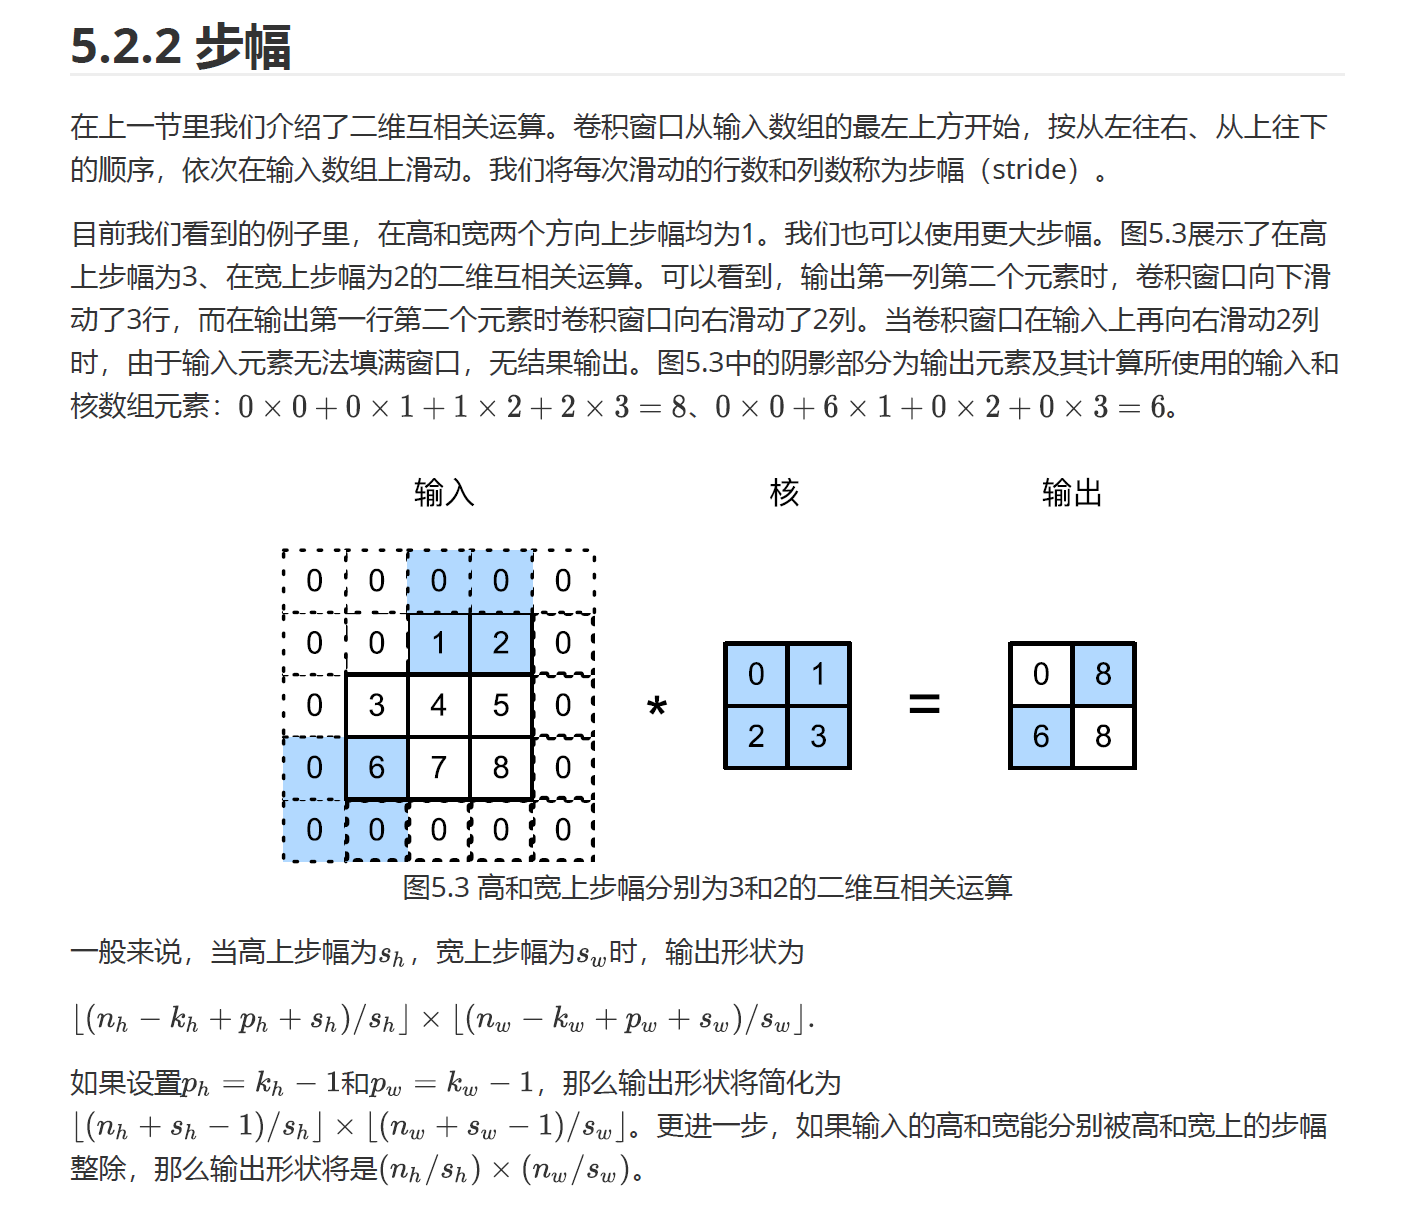
\includegraphics[scale=0.22]{./image/前期总结/DIDL.png}
    \caption{\emph{DiveIntoDeepLearning}中介绍卷积中的步幅概念}
    \label{fig:DIDL}
\end{figure}

此外,在每周的组会报告中,我们都需要阅读有关深度学习及医学图像处理中的相关论文并汇报;同时,也结合CSDN、知乎等平台上对于论文的理解整理笔记;其中包括但不限于:\emph{U-Net: Convolutional Networks for Biomedical Image Segmentation},\emph{Deep Semantic Segmentation of Natural and Medical Images: A Review}等,在这个过程中,我们对冠脉分割的发展历程、研究现状以及未来可能的发展方向有了大致的把握。

\begin{figure}[H]
    \centering
    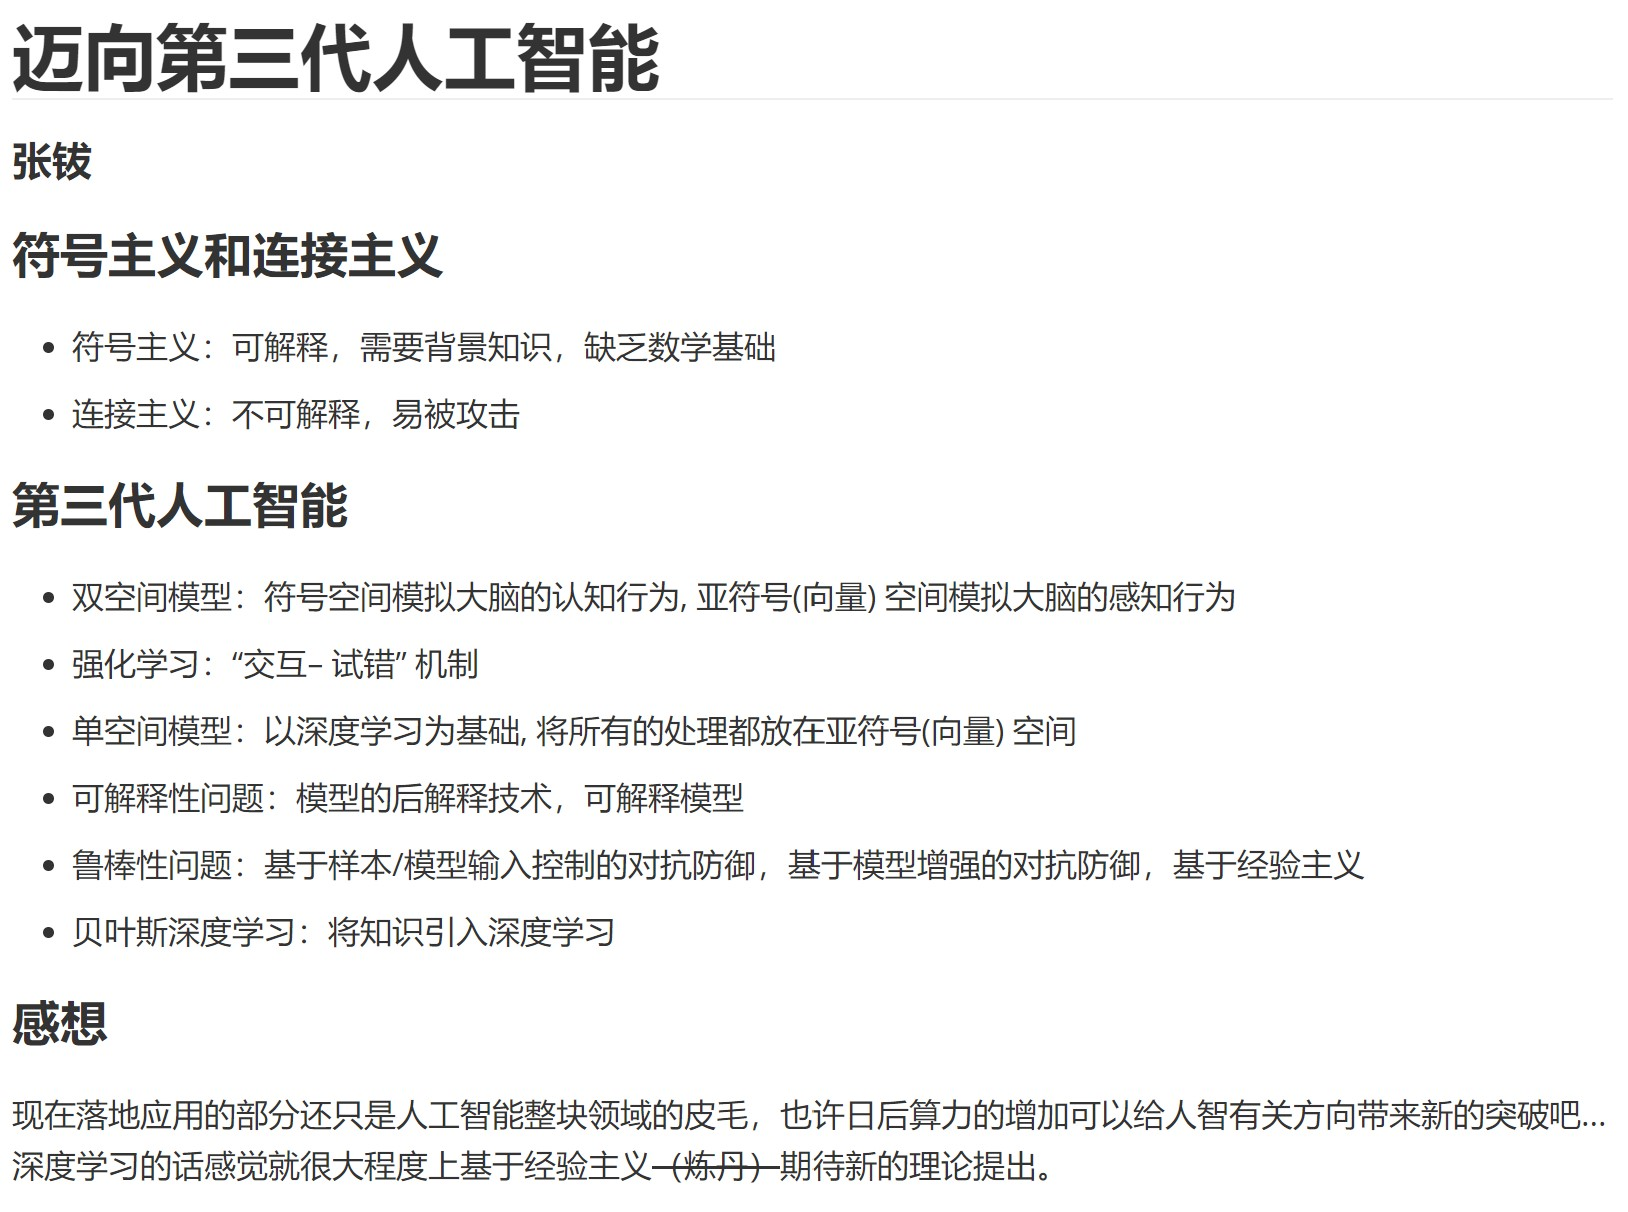
\includegraphics[scale=0.5]{./image/前期总结/Note.jpg}
    \caption{论文阅读笔记}
    \label{fig:Note}
\end{figure}

在基础环境配置方面,主要是Pytorch+Pycharm的本地环境配置和云端服务器连接配置;使用并配置Xshell7连接九龙湖服务器并使用显卡进行模型测试。同时安装Mavislab用于医学图像的预览和结果分析。

\begin{figure}[H]
    \centering
    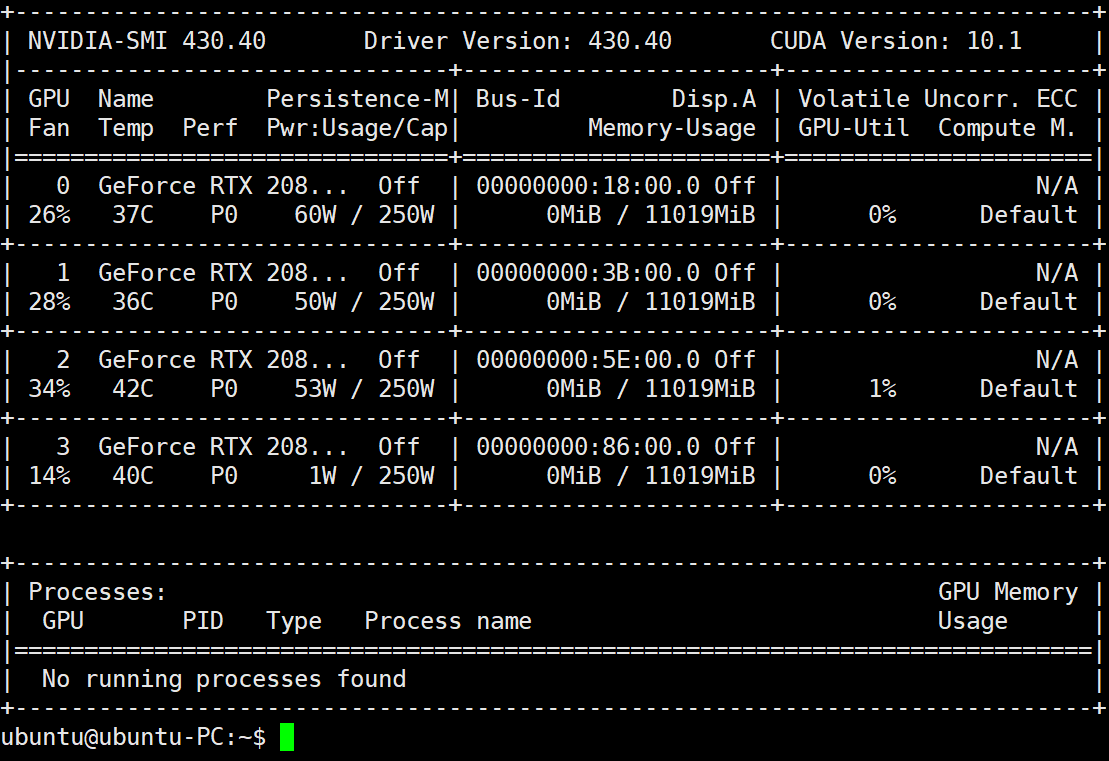
\includegraphics[scale=0.3]{./image/前期总结/Server.png}
    \caption{云服务器连接}
    \label{fig:Server}
\end{figure}

\subsubsection{第二阶段:简单算法编写\&神经网络训练实操}

一个完整的深度学习模型主要包括:数据预处理、网络结构设计、训练流程设计和预测反馈等部分。基于上述分块,我们分阶段地完成了相关工作,并在最后整合处理。

第一周我们首先熟悉了numpy 库,神经网络torch库,numpy 与torch之间的转换;实现图像数据的读取,存储,能够裁剪指定大小的图像,更改图像数据类型,更改图像的维度;最后实现DataLoader部分代码;

第二周我们自行编写了UNet网络框架了,加深了对于正则化、RELU函数、Dropout、上下采样的理解;

第三周我们实现了不同损失函数的设计,并基于算法完成了DO-Layer部分的编写从而解决了动态不平衡问题;

之后我们上述部分,完成了剩余部分的编写,用image\_ROI中的图像作为输入,label\_ROI中的图像作为标签,用Unet作为基础网络,交叉熵作为基础损失,实现具体的分割任务,并测试Dice系数。

\begin{figure}[H]
    \centering
    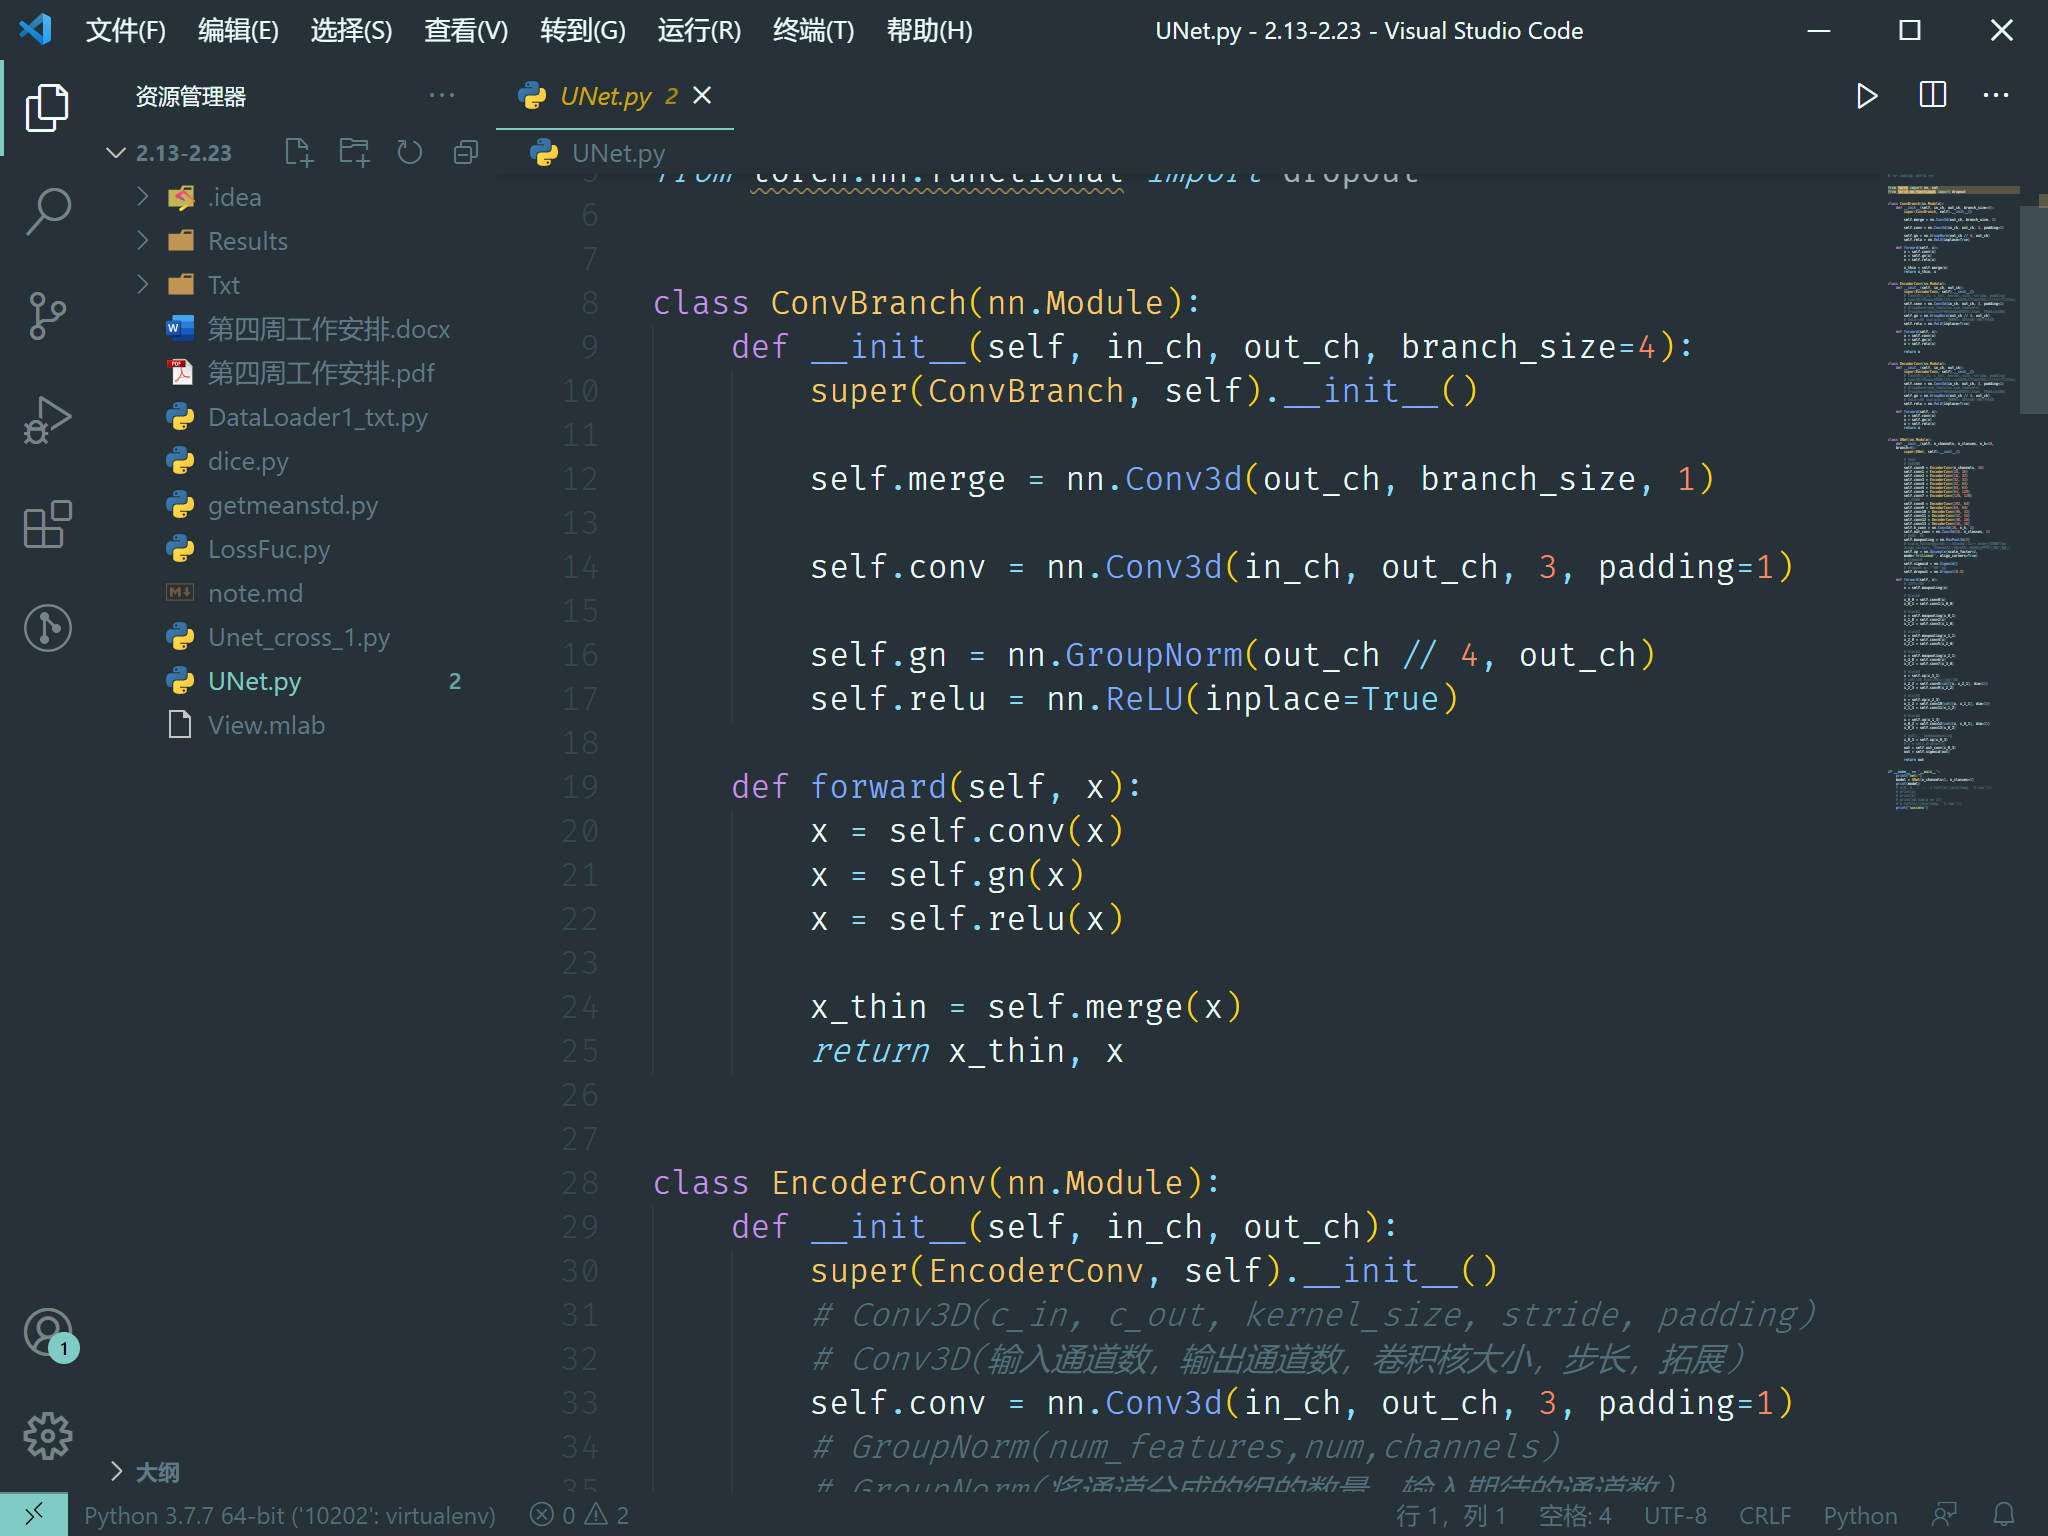
\includegraphics[scale=0.15]{./image/前期总结/Code.png}
    \caption{部分代码展示}
    \label{fig:Code}
\end{figure}

\subsubsection{第三阶段:算法化改进\&结果分析讨论}

未加改进的经典Unet网络训练的分割结果不是很理想,而且使用全监督方法,在冠脉标注难以大量手动获得的背景下,该网络的发展前景和潜力不足。我们希望用较少的标注数据训练出分割效果较好的神经网络,于是我们采用考生-考官训练模型(Examinee-Examiner Network)来进行训练。在此模型中,考生网络是根据管腔标签对原心脏CT图像进行分割预测的主体;而考官网络负责学习管腔标签和高斯增强后中心线标签之间的映射关系,作为前提条件。在此基础上,经训练后的考官网络可用来评估考生网络的预测输出成果,并反馈至后者,达到监督训练考生网络的目的。

首先,我们采用了两份数据集:

\begin{itemize}
    \item \textbf{Cardiac CCTA Data}
    数据来源于数据集为132例主心外膜冠状动脉有狭窄的患者的心脏CCTA图像,该影像由上海交通大学附属第六人民医院、首都医科大学附属北京安贞医院提供。这些CCTA数据由来自上海交通大学Med-X研究所的影像核心实验室的经验丰富的分析师注释,另有一位在心脏成像方面有10年经验的资深专家对注释数据集进行质量控制。原始图像大小为512*512每片,每张图像有200-500张切片。
    \item \textbf{ASOCA Data} 
    该数据集来源于2020年MICCAI“冠状动脉自动分割”挑战赛。他们提供了40张使用造影剂显示冠状动脉的CCTA图像,包括20名健康人士和20名冠状动脉疾病患者,并由三位专家注释员对该数据集进行注释。
\end{itemize}

其次,本项目所用神经网络都采用U-net的结构。U-net是一个在全卷积神经网络的基础上改进优化的网络结构,由特征提取收缩路径和上采样扩张路径组成,整体类似于英文字母U,因而得名。由于医学图像语义简单、结构固定,高级语义信息和低级特征都很重要,而U-net通过底层信息和高层信息结合,能够显著提高分割的精度。根据训练需要,考生网络采用4层U-net,考官网络采用3层。训练时通过计算平衡交叉熵损失函数(Balanced Cross-Loss)来不断更新调整网络权重参数,从而训练网络提高分割结果的准确性。

\begin{figure}[H]
    \centering
    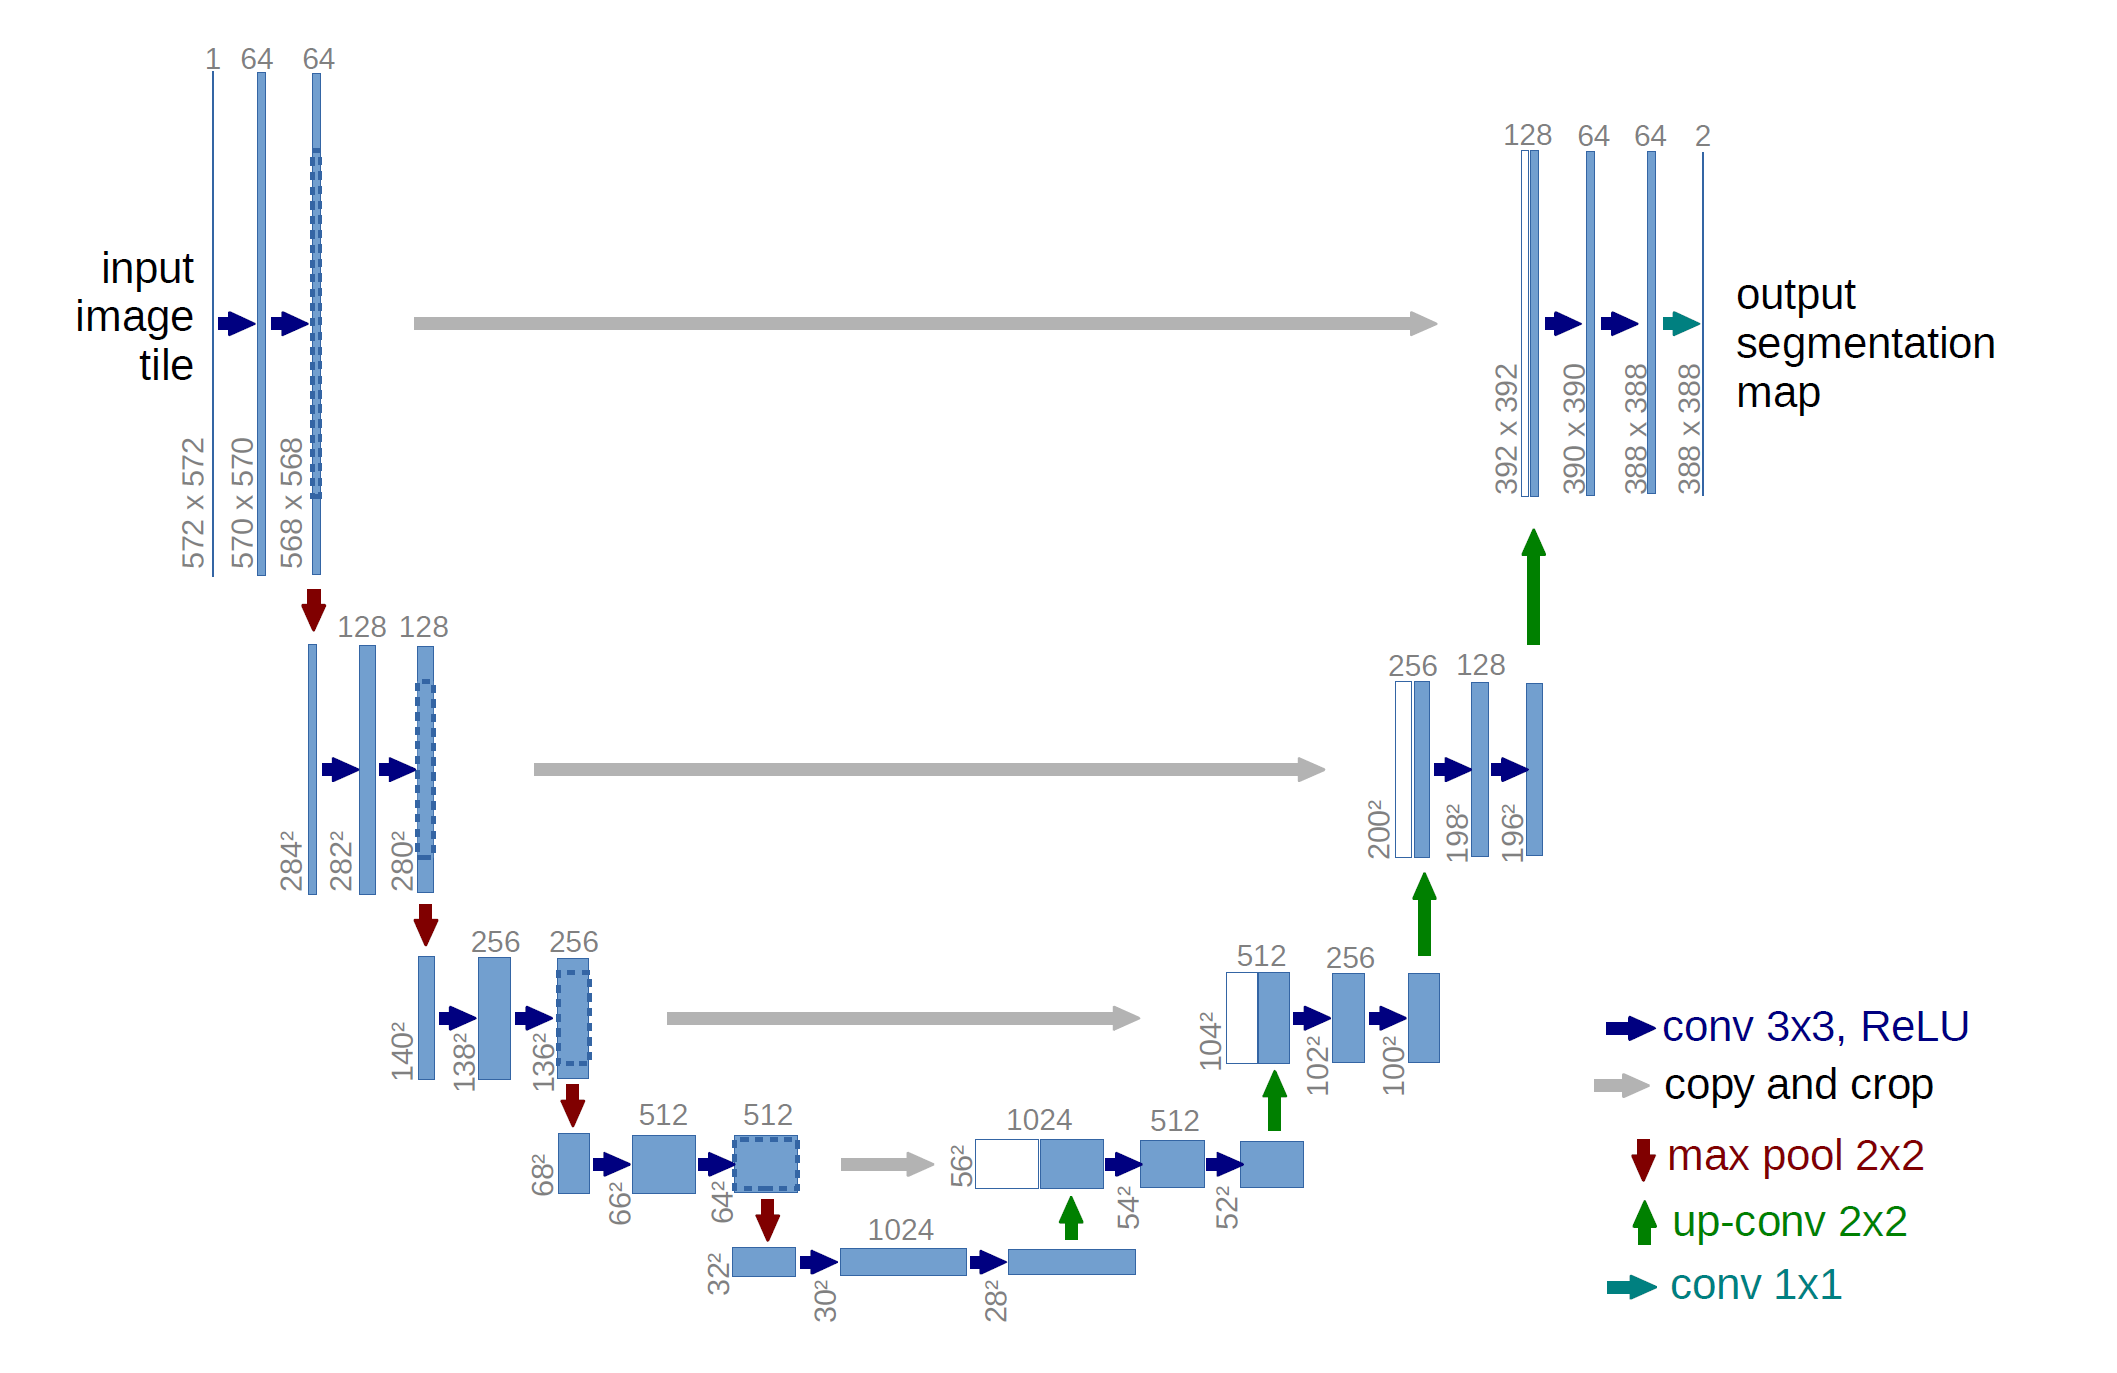
\includegraphics[scale=0.15]{./image/前期总结/Unet.png}
    \caption{Unet网络结构图}
    \label{fig:Unet}
\end{figure}


在考官网络中,采用全监督学习,以冠脉管腔标签为输入,高斯增强的冠脉中心线信息为标签进行训练,计算损失函数,令其学习管腔拓扑结构的特征。与此同时,在考生网络中输入心脏原图像,以管腔标签作为约束,将考生网络的分割结果与标签计算损失,反馈至考生网络。最后,将考生网络输出的冠脉分割结果作为输入送到考官网络中,令经受训练的考官网络对其进行评估和优化,再次通过损失函数反作用于考生网络。如此结合了管腔分割特征训练和考官网络评估反馈,对考生网络实现了效果较好的弱监督图像分割学习。

\begin{figure}[H]
    \centering
    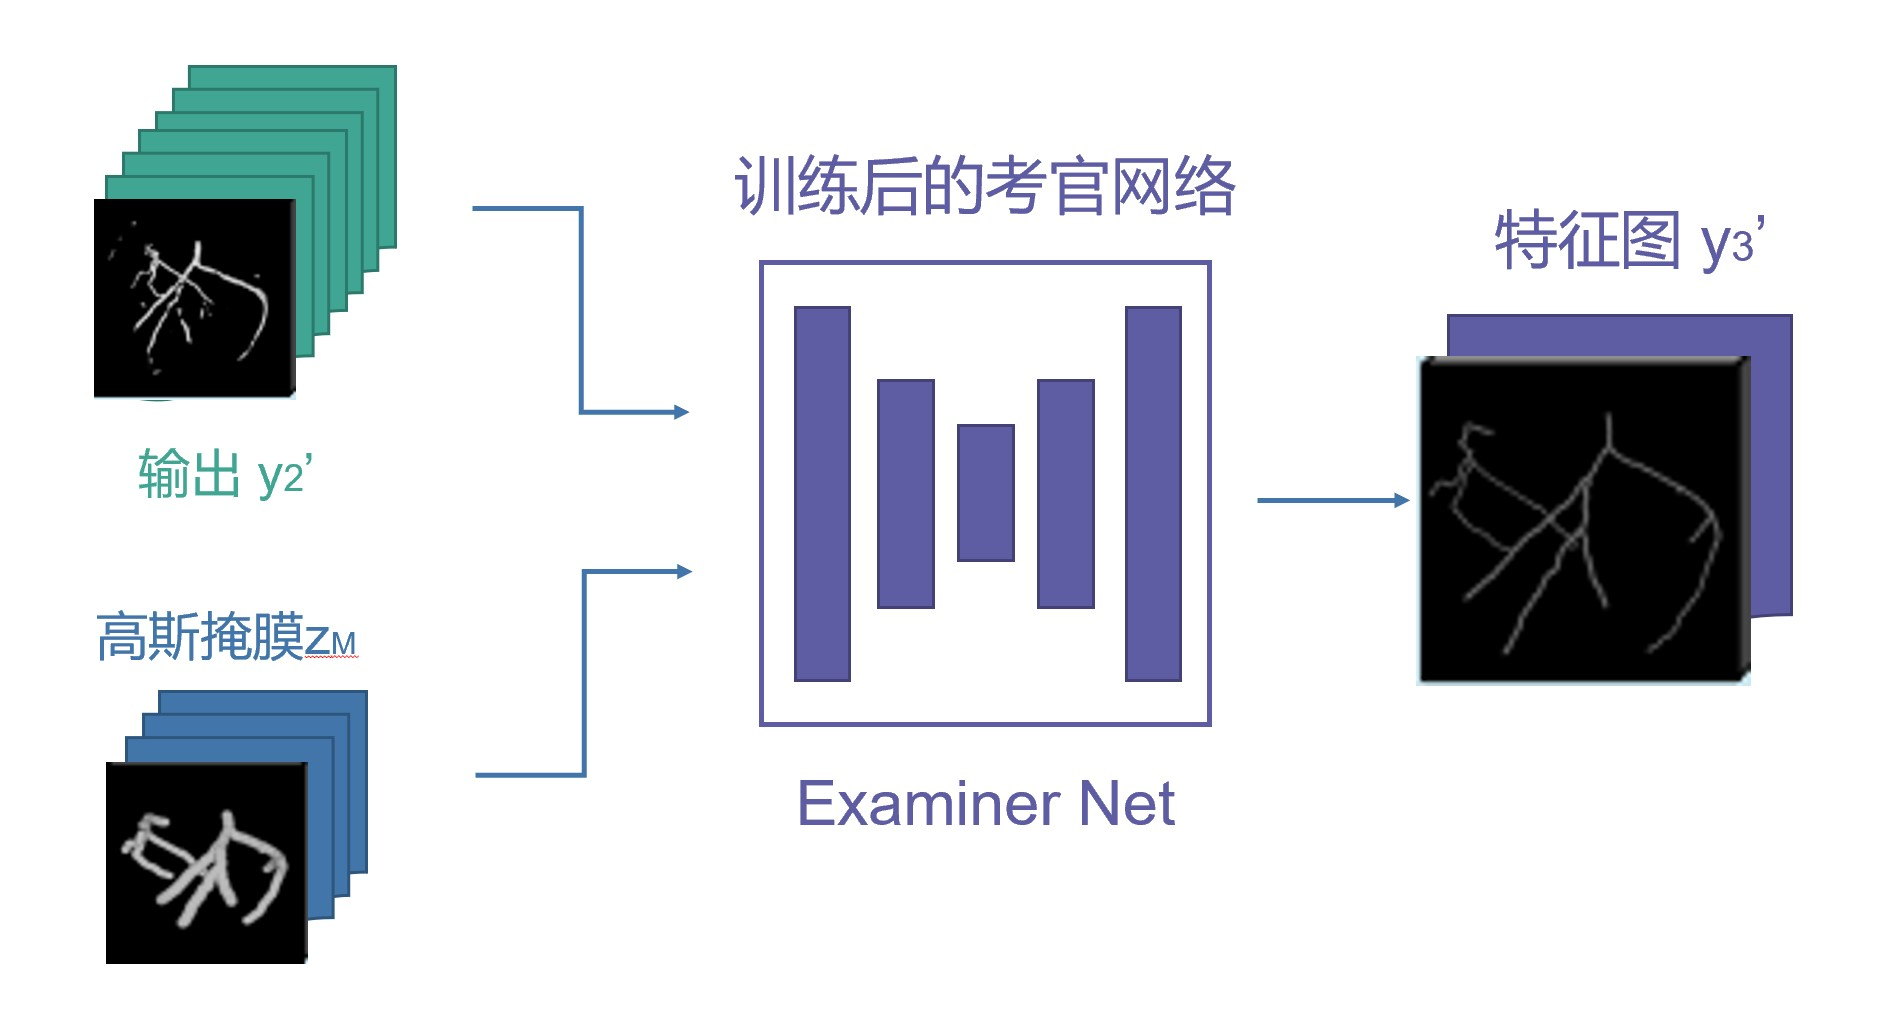
\includegraphics[scale=0.5]{./image/前期总结/EENet.jpg}
    \caption{EE-Net算法流程图}
    \label{fig:EENet}
\end{figure}


此方法相比以原图像作为输入的全监督学习,所需标签训练集显著减少,符合我们的设计理念。同样是150轮训练的结果,而且只使用了很少的冠脉标签,新的网络的平均Dice为0.73。

\begin{figure}[H]
    \centering
    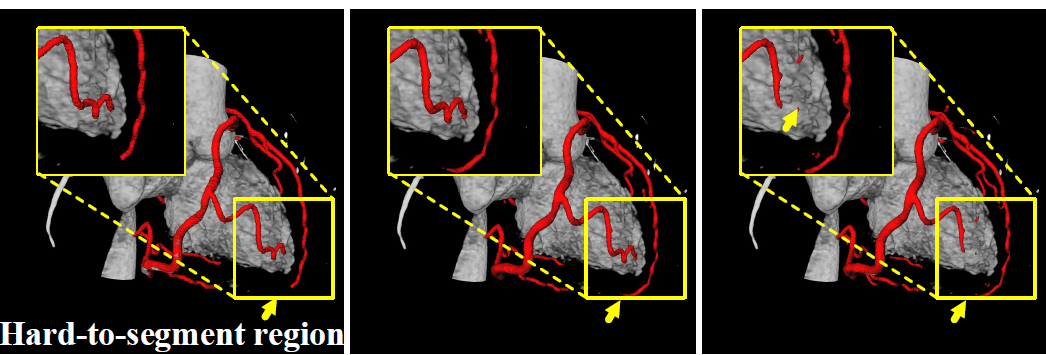
\includegraphics[scale=0.5]{./image/前期总结/Result.png}
    \caption{左侧为标签,中间为EENet运行结果,右侧为注意力UNet;可以看到EE-Net的分割基本没有出现断裂;}
    \label{fig:Result}
\end{figure}

\subsubsection{第四阶段:竞赛准备\& GUI界面编写调试}

为了验证算法的优越性并以赛促研,我们将算法即整体流程封装,基于PyQt5+Mayavi可视化平台,形成”ArteryLumenSeg“可视化应用程序,并参加2021届计算机设计大赛人工智能赛道。程序包含“导入图片”、“查看3D视图”、“查看2D切片”、“查看图片标签”、“预测图片标签”、“保存预测标签”功能模块,图像渲染清晰直观,可以让使用者清楚看到心脏冠脉管腔的位置、粗细等信息,而且可以对没有管腔标签的图片进行预测,一定程度上解决了管腔标签稀少带来的问题。

\begin{figure}[H]
    \centering
    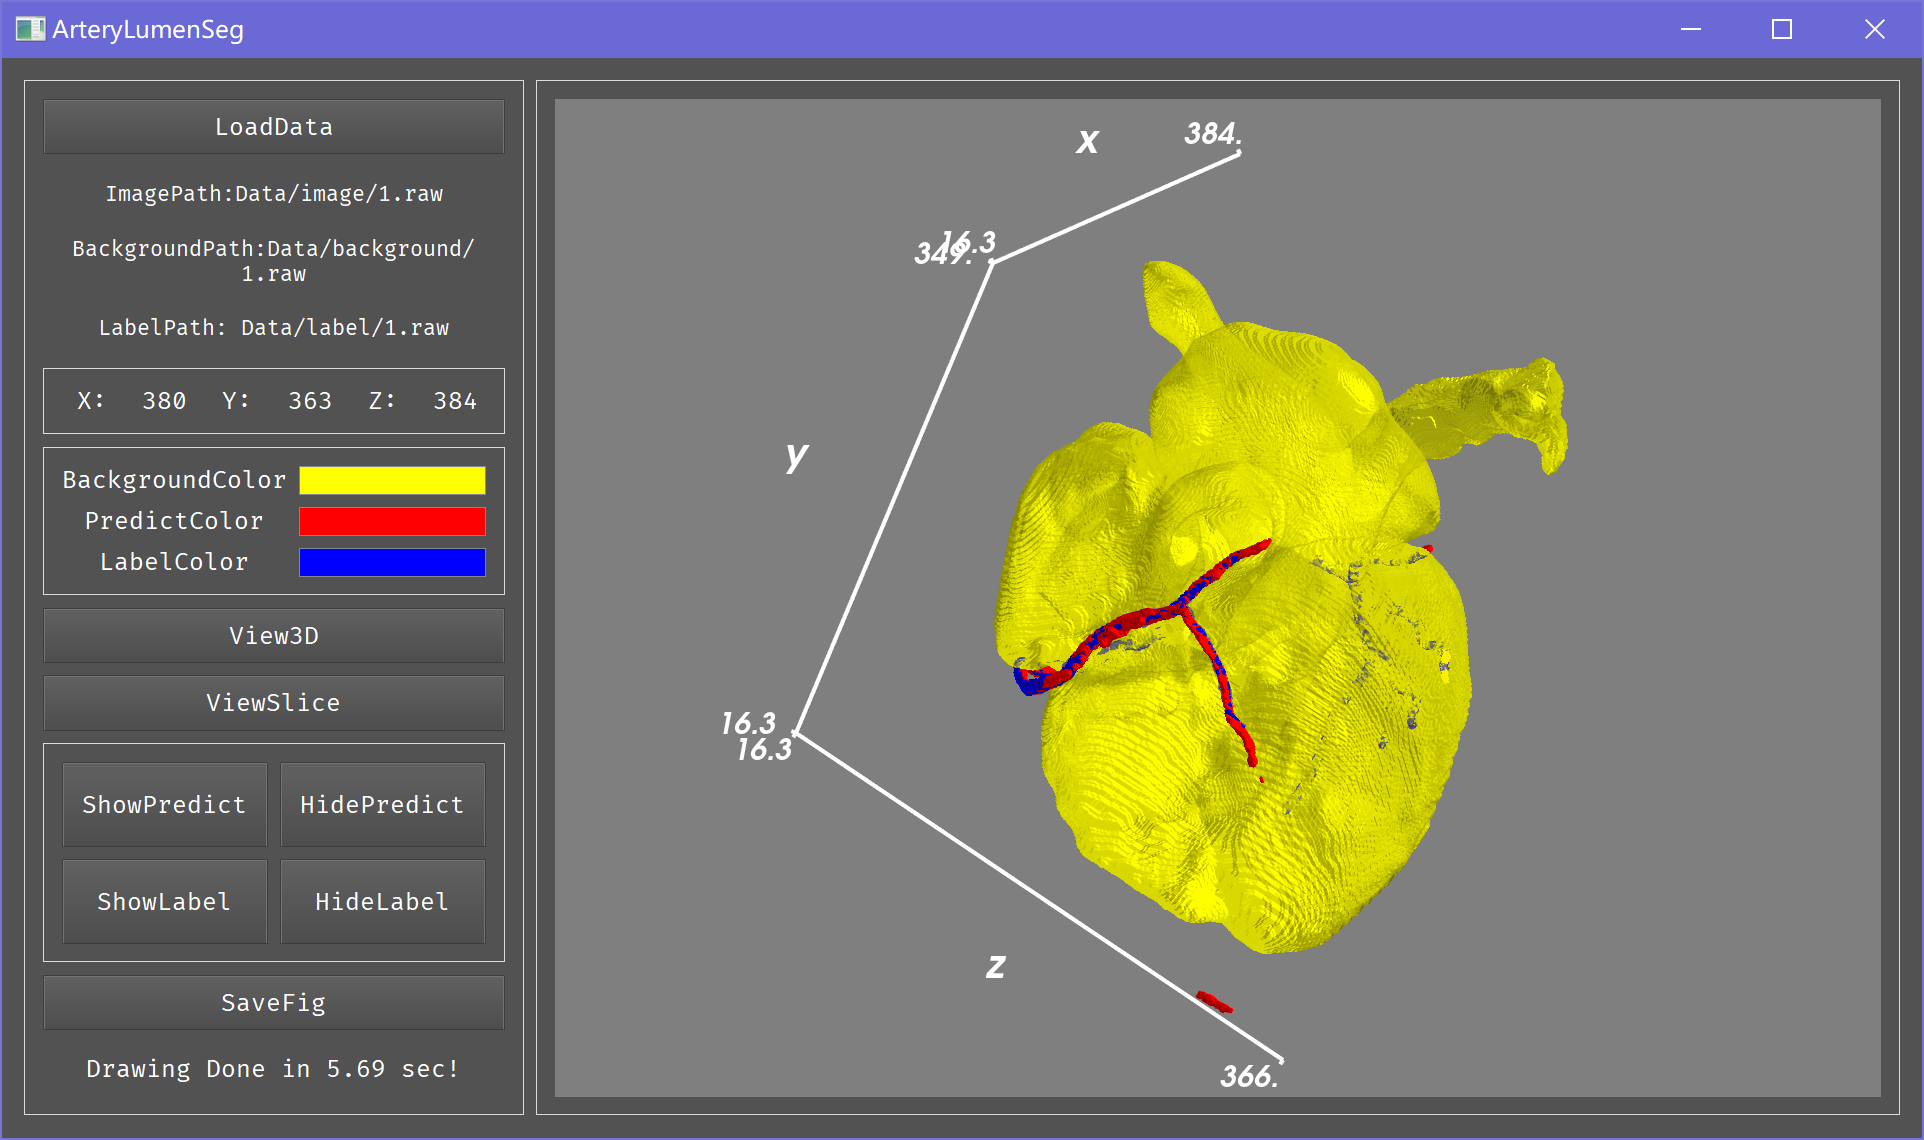
\includegraphics[scale=0.2]{./image/前期总结/GUI.png}
    \caption{GUI界面演示}
    \label{fig:GUI}
\end{figure}


具体操作流程为:

\begin{itemize}
    \item 点击LoadData按钮,选择训练样本图片.raw文件,程序会自动从对应的文档读取对应的支持文件,并将对应文件的路径及训练样本的尺寸显示在界面上;
    \item 点击View3D按钮,程序会根据读入的数据绘制心脏3D图;根据电脑性能及图片规模,加载需要一定时间;加载完成后,下方会提示加载完成并输出加载时间;
    \item 点击ShowPredict按钮,程序会根据训练样本和训练好的网络输出预测的冠脉分割结果,标记为红色;程序下方会提示当前进度并输出运行时间;拖动界面中的图片,可以从不同角度预览3D分割结果,并可进行缩放、旋转等操作;
    \item 点击ShowLabel按钮,程序会绘制冠脉分割标签,标记为蓝色;
    \item 点击HidePredict或者HideLabel按钮,可以隐藏对应的分割结果,便于观察;
    \item 点击SaveFig按钮,程序会将预览的结果保存到对应目录中,便于日后查阅;
    \item 点击ViewSlice按钮,界面会清空已绘制的图像并绘制XYZ方向的心脏三维切片图;通过鼠标拖动对应切片可以观察不同层次的图像结果;
\end{itemize}

\begin{figure}[H]
    \centering
    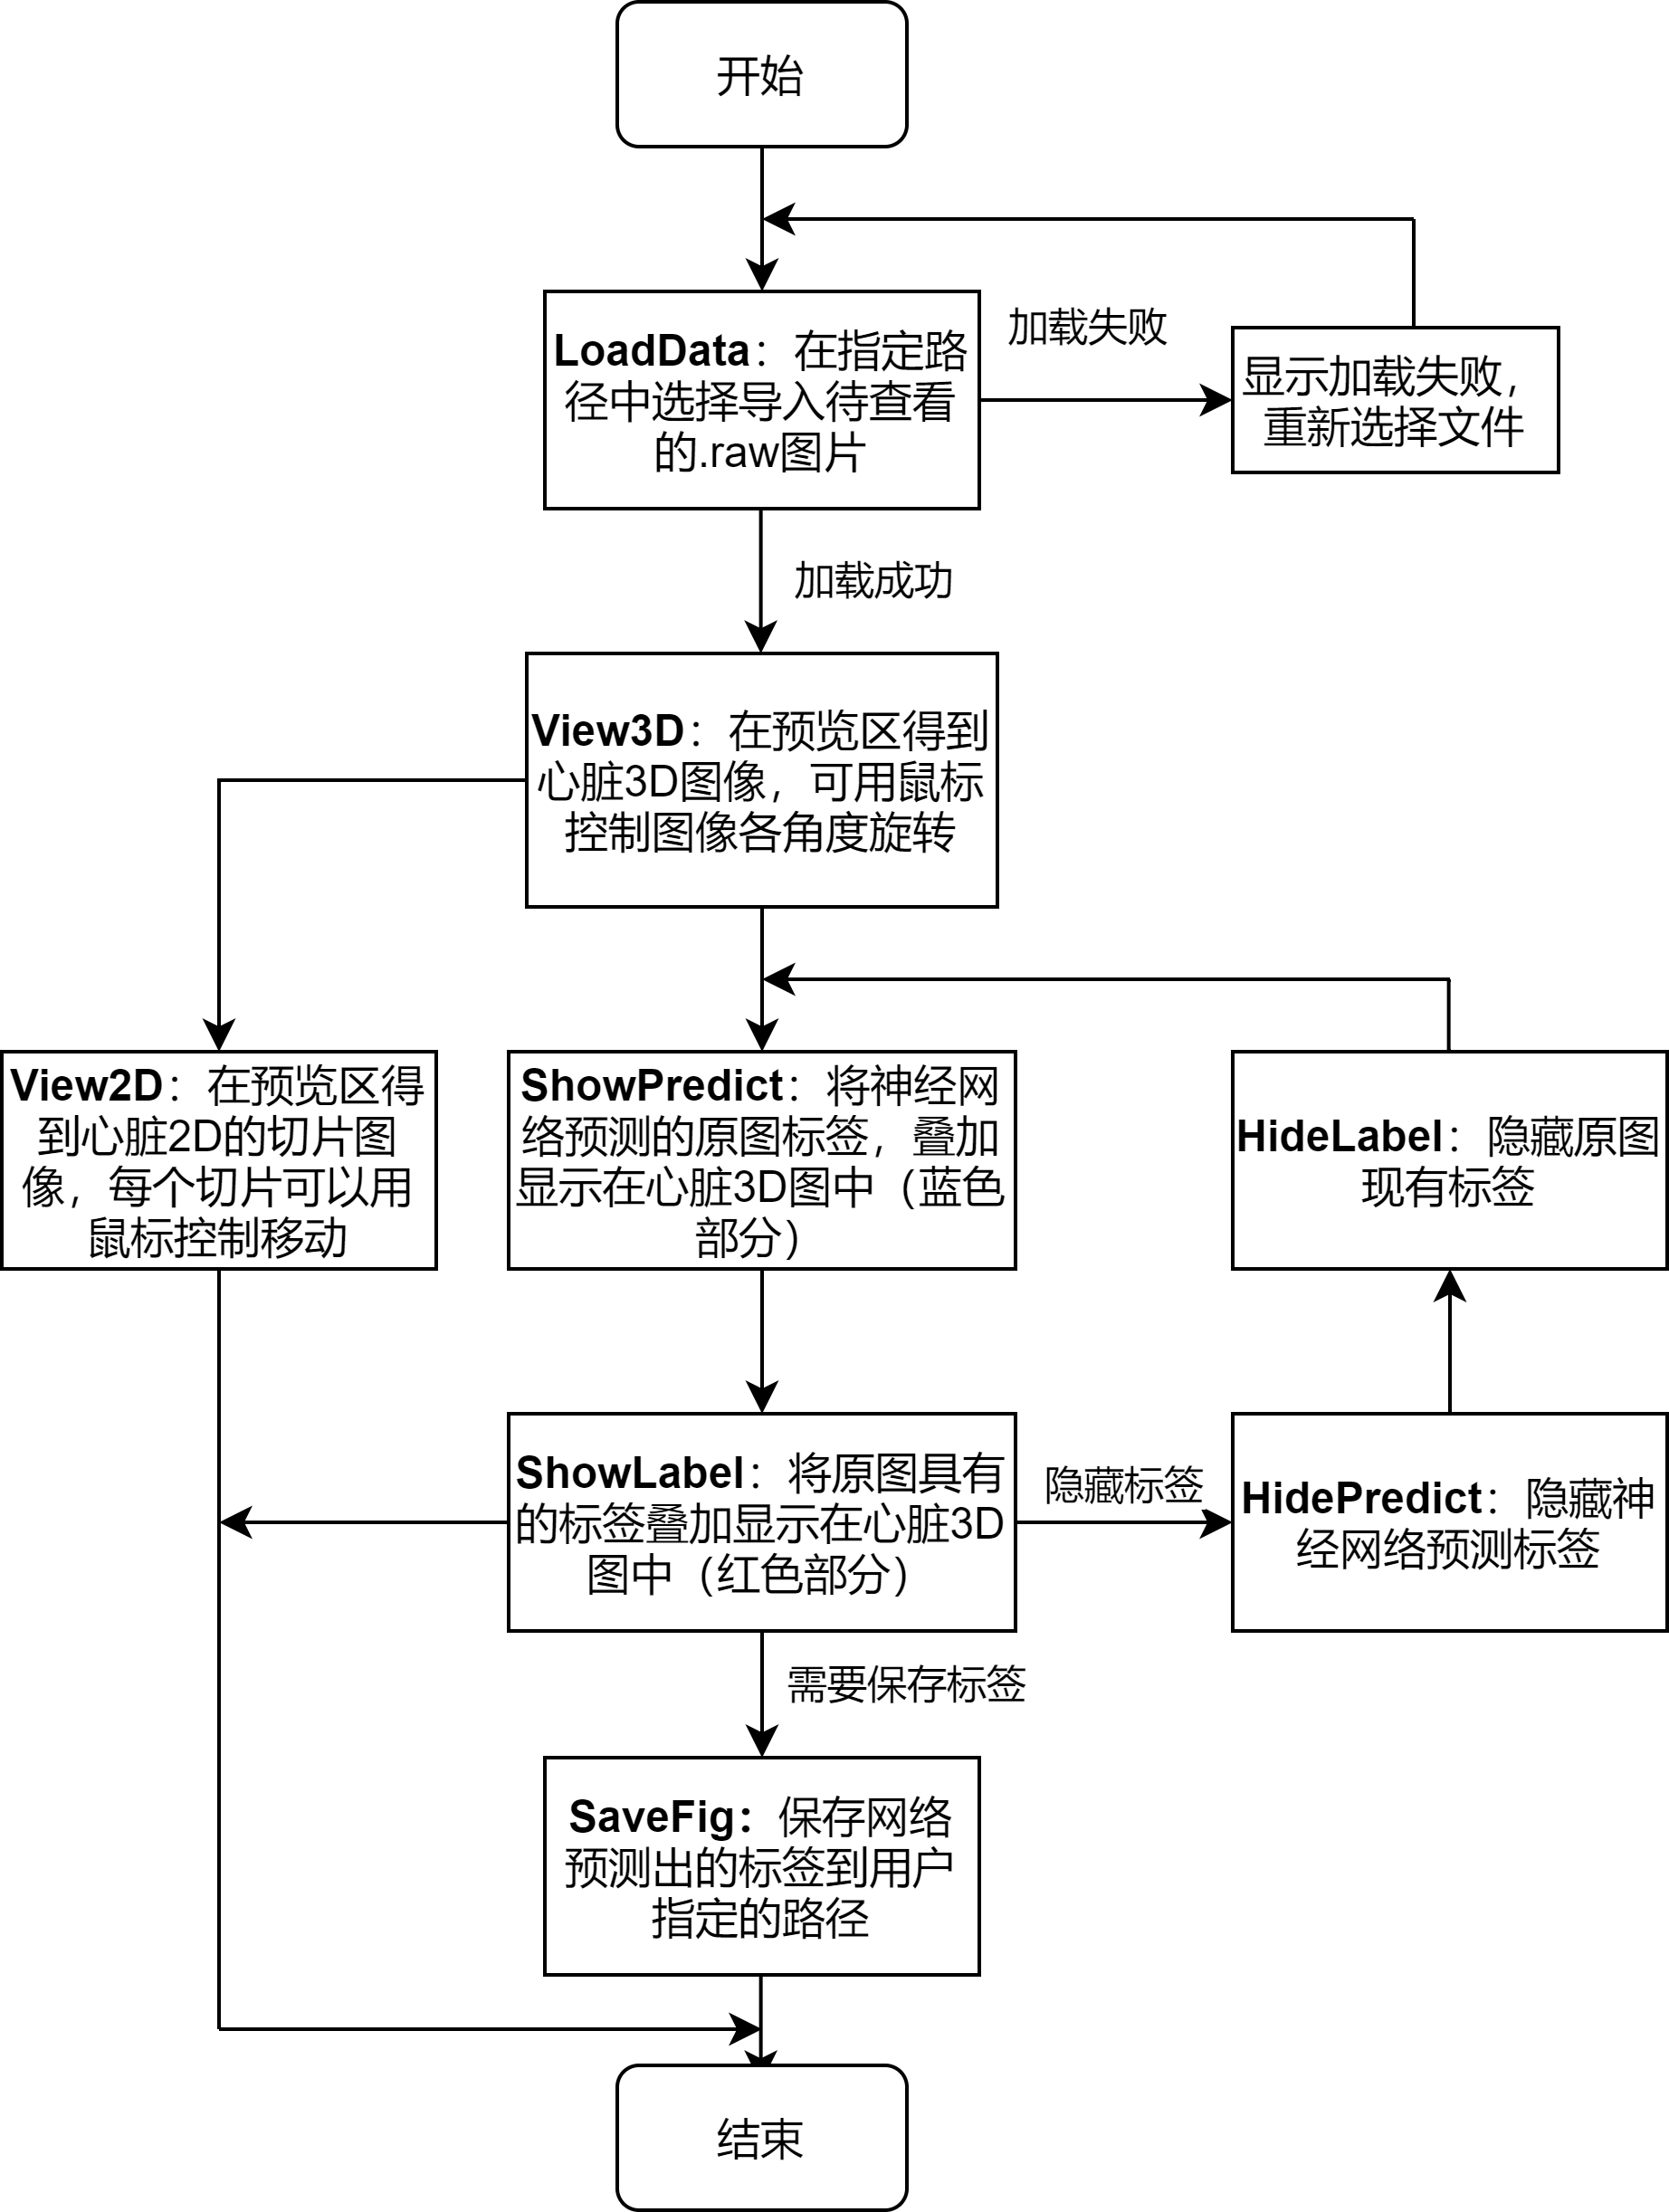
\includegraphics[scale=1]{./image/前期总结/GUIDiagram.png}
    \caption{GUI运行流程图}
    \label{fig:GUIDiagram}
\end{figure}

基于上述成果,我们对GUI的整体操作过程制作了宣传视频并配以解说。

\subsection{项目取得成绩}
本项目参与校2021届计算机设计大赛人工智能赛道并取得了优秀的初赛成绩,现已被推荐至省赛;

\subsection{项目实际进度与预期}
我们的实际进度与项目预期的中期进度基本持平,但在GUI的细节优化和算法的后处理部分仍有欠缺。这是我们后期工作仍需完善的;

\subsection{项目开展遇到的问题}

\begin{itemize}
    \item GUI界面中多线程绘图与Mayavi的兼容性有待研究;
    \item GUI中2D视图与鼠标交互部分;
    \item 算法中分割断裂部分和误分割部分的后处理;
\end{itemize}

\section{项目后期工作展望}

我们的项目实际进度已实现多数功能,但深度学习算法和可视化GUI部分仍有进一步完善的空间。为打造可用性更好、调用更方便、准确度更高的“一体化”诊断平台,本项目拟从以下具体方面进行后续研究。

\subsection{GUI方向}

Mevislab作为一款医学图像处理软件,其界面清晰直观、操作简单,是其在医学图像领域收到广泛青睐的原因之一。本项目的可视化目标是加入Mevislab图像显示的部分功能,如拖动鼠标调整亮度、在鼠标所在坐标位置显示亮度参数等等。同时界面上会添加新的视图,包括图像的XY切面、XZ切面、YZ切面、和3D图像展示,便于观察比对。此外,我们将尝试多线程非阻塞加载原图、标签的方法,并采用降采样的方法,优化运行速度,防止界面意外卡死。之后利用连通域相关算法,对图像与标签做后处理,从而排除网络误分割部分,达到更好的显示效果。最后,根据工作需要添加功能,实现医学图像处理的自动化、高度可视化,增强软件的普适性,从而提高科研工作者的工作效率和体验;在上述工作完成后,考虑申请软件著作权。

\subsection{深度学习算法方向}

目前我们的算法已完成图像的冠脉管腔分割部分,效果良好;因此,接下来我们预计在此基础上继续优化,采取优化从而提高精确度。主要思想有:

\paragraph{深度监督}
所谓深度监督(Deep Supervision),就是在深度神经网络的某些中间隐藏层加了一个辅助的分类器作为一种网络分支来对主干网络进行监督的技巧,用来解决深度神经网络训练梯度消失和收敛速度过慢等问题。通常而言,增加神经网络的深度可以一定程度上提高网络的表征能力,但随着深度加深,会逐渐出现神经网络难以训练的情况,其中就包括像梯度消失和梯度爆炸等现象。为了更好的训练深度网络,我们可以尝试给神经网络的某些层添加一些辅助的分支分类器来解决这个问题。这种辅助的分支分类器能够起到一种判断隐藏层特征图质量好坏的作用。

\begin{figure}[H]
    \centering
    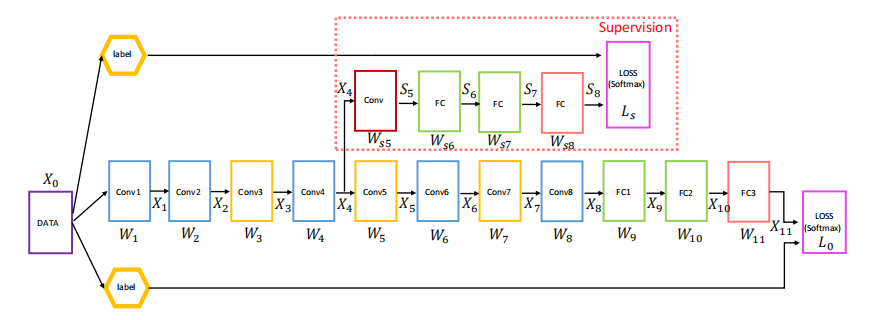
\includegraphics[scale=0.8]{./image/后期展望/8-layer.png}
    \caption{深度监督网络结构示意图\cite{24}}
    \label{fig:DeepSupervision}
\end{figure}

\paragraph{领域知识嵌入}
在使用传统的深度学习网络对病灶进行分割时,网络均只考虑了本身图像上的信息,让网络本身通过大量的图像与标签的对应关系,进行深度学习模型的训练。这一系列过程中没有任何人工的干预以及人为的先验信息。当数据量十分巨大时,这种做法往往能够取得非常好的分割效果,但当数据量相对较小时,如很多医学影像数据往往只有几十张精准标注的图像,引入医生本身的解剖学信息往往能够取得更好的分割效果。但问题的难点在于如何将医生的临床知识进行量化表示,并与深度学习的分割相结合。如何将医学中繁杂多样的领域知识与深度学习训练结合从而使网络更好的识别对应区域从而达到更好的分割效果也是我们接下来要思考的方向之一;目前主要的研究思路包括:

\begin{itemize}
    \item 不同形式的先验知识形式;如树状/管状结构、位置信息、亮度信息等;
    \item 先验知识的不同嵌入方法:特征提取的浅层网络网络、图卷积网络、贝叶斯形式的嵌入、与深度监督的结合;
\end{itemize}

\begin{figure}[H]
    \centering
    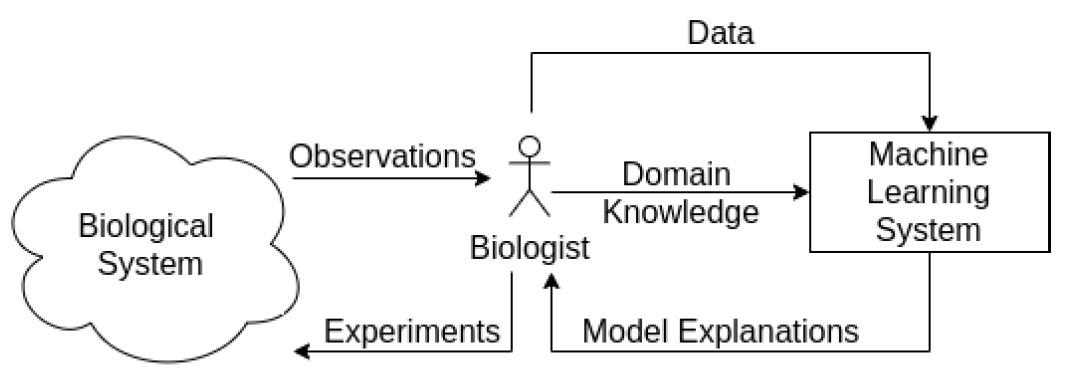
\includegraphics[scale=0.6]{./image/后期展望/DomainKnowledge.jpg}
    \caption{医学领域知识嵌入的思想\cite{25}}
    \label{fig:DomainKnowledge}
\end{figure}

\paragraph{损失函数设计}
新的损失函数;损失函数是深度学习的灵魂所在;能否在当前框架的基础上,以任务导向为核中心,优化损失函数从而更精确的分割,从而增强网络的泛化能力是我们可以思考的方向,其中包括:

\begin{itemize}
    \item 加入重叠度量函数作为加权正则项
    \item 考生和考官网络使用不同的损失函数
    \item 有标签和无标签数据使用不同的损失函数
    \item 将一些传统的算法思路加入卷积神经网络中
    \item 搜索边缘算子的损失函数方法
\end{itemize}

\begin{figure}[H]
    \centering
    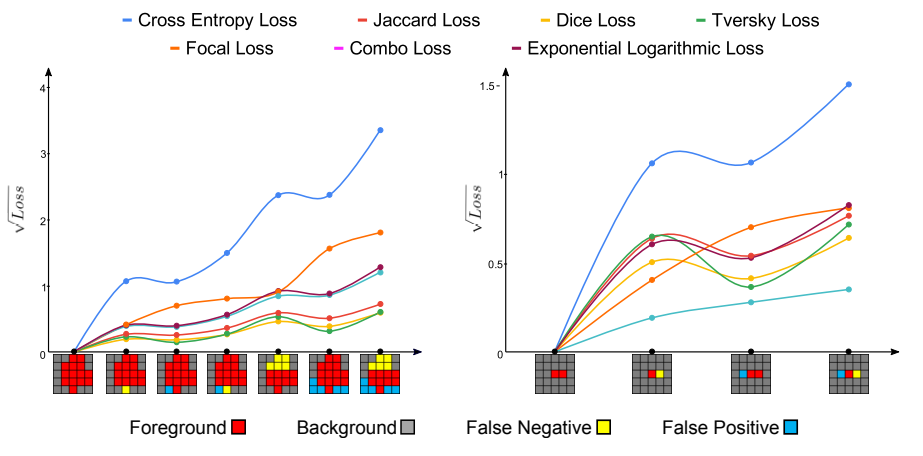
\includegraphics[scale=0.6]{./image/后期展望/LossFunc.png}
    \caption{不同损失函数的在不同环境下的性能对比\cite{26}}
    \label{fig:LossFunc}
\end{figure}

\paragraph{狭窄检测}
由于对细小管腔部分进行狭窄检测也是冠脉提取的重点之一,因此本项目拟继续从深度学习思想出发,阅览相关论文,学习并搭建成型的狭窄检测算法,在数据集中应用。

\section{经费使用情况}

\begin{itemize}
    \item 书籍购买 500元 
    \item 移动硬盘(数据存储)500元 
    \item 资料打印费 200元
\end{itemize}

\bibliography{wpref}

\end{document}
